% 1. ročník MAT – příprava 96; inspirace Realisticky.cz 020501–020506, úlohy nově sestavené.
\documentclass[11pt,a4paper]{article}
\input{../../sablony/pripravy/priprava.sty}
\usepackage{tikz}
\usepackage{pgfplots}
\pgfplotsset{compat=1.18}
\usetikzlibrary{arrows.meta}
\nastavPripravu{1. ročník}{Kvadratické funkce}{96}{Úvod do kvadratické funkce}
\begin{document}
\blok{Od přímky k parabole}
Při vzorci $y=x^2$ se výstup při zvětšení $x$ o jednotku nemění o stále stejné číslo: pro $x=0,1,2,3$ dostáváme $0,1,4,9$. Graf proto není přímka.\par
Obsah čtverce $S=a^2$ je motivací pouze pro $a\ge0$; matematická funkce $y=x^2$ je naopak definována pro všechna reálná $x$.
\begin{definiceBox}
\textbf{Kvadratická funkce} je funkce daná předpisem
\[f(x)=ax^2+bx+c,\qquad a,b,c\in\mathbb R,\quad a\ne0,\]
s definičním oborem $D(f)=\mathbb R$. Jejím grafem je \textbf{parabola}.
\end{definiceBox}
\blok{Základní parabola $y=x^2$}
Vyplníme tabulku (stejné hodnoty pro opačná $x$):
\[\begin{array}{c|rrrrrrr}x&-3&-2&-1&0&1&2&3\\\hline x^2&9&4&1&0&1&4&9\end{array}\]
Zaneseme body do soustavy souřadnic a spojíme je plynulou křivkou; parabola se neskládá z rovných úseček.
\begin{center}
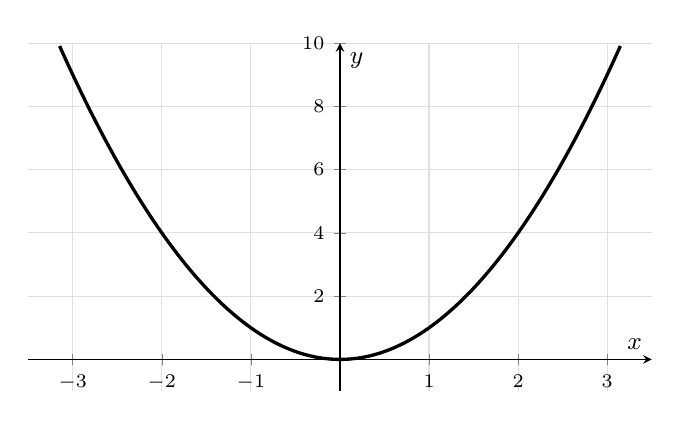
\begin{tikzpicture}
\begin{axis}[
width=9.5cm,height=6.0cm,axis lines=middle,
xmin=-3.5,xmax=3.5,ymin=-1,ymax=10,
xtick={-3,-2,...,3},ytick={0,2,4,6,8,10},grid=both,
minor tick num=0,grid style={black!12},
tick label style={font=\scriptsize},xlabel={$x$},ylabel={$y$},
label style={font=\small},restrict y to domain=-1:10,
clip=true,legend style={font=\scriptsize,draw=none,fill=none,at={(0.98,0.98)},anchor=north east},
]
\addplot[very thick,solid,domain=-3.5:3.5,samples=160] {x^2};
\end{axis}
\end{tikzpicture}
\end{center}
\begin{definiceBox}
U funkce $f(x)=x^2$ je \textbf{vrchol} $V[0;0]$, osa souměrnosti $x=0$,
$D(f)=\mathbb R$ a $H(f)=\langle0;+\infty)$. Funkce je sudá, na $(-\infty;0\rangle$ klesající a na $\langle0;+\infty)$ rostoucí. Nejmenší hodnota je $0$.
\end{definiceBox}
\blok{Společně řešené příklady}

\begin{prikladReseniBox}
Určete hodnoty $f(-3)$, $f(1)$, $f(2)$ pro $f(x)=x^2$. Které dva různé body grafu mají stejnou výšku $4$?
\tcblower
\[
\begin{aligned}
f(-3)&=(-3)^2=9,\qquad f(1)=1,\qquad f(2)=4 \\
x^2&=4\ \Longrightarrow\ x=-2\ \text{nebo}\ x=2 \\
A&[-2;4],\quad B[2;4]
\end{aligned}
\]

\end{prikladReseniBox}
\begin{prikladReseniBox}
Rozhodněte, které předpisy jsou kvadratické: $p(x)=2x^2-3x+1$, $q(x)=x^2-x^2+4$, $r(x)=-x^2$ a $s(x)=3x-1$.
\tcblower
\[
\begin{aligned}
p(x)&=2x^2-3x+1:\ a=2\ne0 \\
q(x)&=4:\ a=0\ \text{-- konstantní} \\
r(x)&=-x^2:\ a=-1\ne0 \\
s(x)&=3x-1:\ a=0\ \text{-- lineární}
\end{aligned}
\]

\end{prikladReseniBox}
\blok{Samostatné procvičování}

\begin{zadaniReseniBox}
a) Doplňte $f(-4)$, $f(-\tfrac12)$ a $f(0)$ pro $f(x)=x^2$.\par
b) Určete všechny hodnoty $x$, pro které $x^2=16$.\par
c) Popište, proč $f(-x)=f(x)$ pro každé reálné $x$.
\tcblower
\[
\begin{aligned}
f(-4)&=16,\quad f(-\tfrac12)=\tfrac14,\quad f(0)=0 \\
x^2&=16\ \Longrightarrow\ x\in\{-4;4\} \\
f(-x)&=(-x)^2=x^2=f(x)
\end{aligned}
\]

\end{zadaniReseniBox}
\blok{Volitelná rezerva}
Uvažujte funkci $S(a)=a^2$ pro délku strany čtverce $a\ge0$. Proč má stejné algebraické pravidlo, ale jiný definiční obor a jiný graf než $f(x)=x^2$ na $\mathbb R$?
\blok{Domácí úkol}
\begin{zadaniReseniBox}[title={Domácí příprava}]
\begin{enumerate}[label=\alph*),itemsep=3pt]
\item Pro $f(x)=x^2$ vypočtěte $f(-5)$, $f(0)$ a $f(\tfrac32)$.
\item Určete všechny body grafu $y=x^2$ s druhou souřadnicí $9$.
\item Pro funkci $y=x^2$ napište $D(f)$, $H(f)$, vrchol a osu souměrnosti.
\item Rozhodněte, zda je $y=x^2$ rostoucí na celé $\mathbb R$. Zdůvodněte pomocí hodnot v $-2,-1,0,1,2$.
\item Které z předpisů $2x^2+1$, $3x-2$, $x(x-1)$, $x^2-(x^2+1)$ jsou kvadratické?
\item Naskicujte $y=x^2$ z bodů pro $x=-2,-1,0,1,2$; vyznačte osu souměrnosti.
\item \textbf{Výzva:} Ověřte algebraicky, zda je $f(x)=x^2$ prostá na $\mathbb R$ a na $\langle0;+\infty)$.
\end{enumerate}
\tcblower
\begin{enumerate}[label=\alph*),itemsep=4pt]
\item
\[
\begin{aligned}
f(-5)&=25,\quad f(0)=0,\quad f(\tfrac32)=\tfrac94
\end{aligned}
\]

\item
\[
\begin{aligned}
x^2&=9\ \Rightarrow\ x=\pm3 \\
A&[-3;9],\quad B[3;9]
\end{aligned}
\]

\item
\[
\begin{aligned}
D(f)&=\mathbb R,\quad H(f)=\langle0;+\infty) \\
V&[0;0],\quad \text{osa: }x=0
\end{aligned}
\]

\item
\[
\begin{aligned}
f(-2)&=4>f(-1)=1>f(0)=0 \\
f(0)&=0<f(1)=1<f(2)=4 \\
\text{Na }\mathbb R&\text{ není monotónní.}
\end{aligned}
\]

\item
\[
\begin{aligned}
2x^2+1&:\ \text{ano};\quad 3x-2:\ \text{ne} \\
x(x-1)&=x^2-x:\ \text{ano} \\
x^2-(x^2+1)&=-1:\ \text{ne}
\end{aligned}
\]

\item
\[
\begin{aligned}
[-2;4],[-1;1], [0;0], [1;1], [2;4] \\
\text{Osa souměrnosti: }&x=0
\end{aligned}
\]

\item
\[
\begin{aligned}
f(-2)&=f(2)=4\ \Rightarrow\ \text{na }\mathbb R\text{ není prostá} \\
0\le x_1<x_2&\ \Rightarrow\ x_1^2<x_2^2 \\
\text{Na }\langle0;+\infty)&\text{ je prostá.}
\end{aligned}
\]

\end{enumerate}
\end{zadaniReseniBox}
\poznamka{Čas: motivace a tabulka 8 min, definice a graf 12 min, dva příklady 12 min, samostatná práce 10 min, závěr 3 min. Pro práci s grafem použij pravítko pouze na osy, nikoliv na parabolu.}
\end{document}
